\section{The quantum Fourier transform and its applications}

In the introduction, we stated that quantum computers can factor numbers much faster than a classical computer. To put this in perspective, finding the prime factorization of an $n$-bit integer is thought to require $exp(O(n^{1/3}\log^{2/3}n))$ operations using the best classical algorithm known, the so-called number \textit{field sieve}. In contrast, a quantum algorithm can accomplish the same task using $O(n^2 \log n \log\log n)$ operations. That is, a quantum computer can factor a number \textit{exponentially} faster than the best known classical algorithms.
\vspace{1em}

But now the question arises, what other tasks a quantum computer can do more efficiently than a classical computer? In this chapter, we talk about the \textit{quantum Fourier transform} which is the key ingredient for quantum factoring and many other interesting quantum algorithms.

\subsection{The quantum Fourier transform}

A very useful and common way to solve a problem in computer science is to break it down or \textit{transform} it into other problem(s) whose solution is known. A great discovery of quantum computation has been that some such transformations can be computed much faster on a quantum computer than on a classical computer.
\vspace{1em}

One such transformation is the discrete Fourier transform. In the usual mathematical notation, the discrete Fourier transform takes as input a vector of complex numbers, $x_0 , \dots , x_{N-1}$ where the length $N$ of the vector is a fixed parameter. It outputs the transformed data, a vector of complex numbers $y_0,\dots,y_{N−1}$, defined by
$$y_k \equiv \frac{1}{\sqrt{N}}\sum_{j=0}^{N-1}{x_j e^{2\pi ijk/N}}$$

The quantum Fourier transform is exactly the same transformation, although the conventional notation for the quantum Fourier transform is somewhat different. The quantum Fourier transform on an orthonormal basis $\ket{0},\dots, \ket{N - 1}$ is defined to be a linear operator with the following action on the basis states,
$$\ket{j} \rightarrow \frac{1}{\sqrt{N}}\sum_{j=0}^{N-1}{e^{2\pi ijk/N}\ket{k}}$$

Equivalently, the action on an arbitrary state may be written
$$\sum_{j=0}^{N-1}{x_j\ket{j}} \rightarrow \sum_{k=0}^{N-1}{y_k\ket{k}},$$
where the amplitudes $y_k$ are the discrete Fourier transform of the amplitudes $x_j$. Now we shall demonstrate the unitarity of the Fourier transform by constructing a manifestly unitary quantum circuit computing the Fourier transform.
\vspace{1em}

In the following, we take $N = 2^n$, where n is some integer, and the basis $\ket{0},\dots , \ket{2^n-1}$ is the computational basis for an $n$ qubit quantum computer. It is helpful to write the state $\ket{j}$ using the binary representation $j = j_1j_2\dots j_n$. More formally, $j = j_1 2^n−1 + j_2 2^n−2 + \dots + j_n 2^0$ . It is also convenient to adopt the notation $0.j_lj_{l+1}\dots j_m$ to represent the binary fraction $j_l/2 + j_{l+1}/4 + \dots + j_m/2^{m-l+1}$.
\vspace{1em}

With a little algebra the quantum Fourier transform can be given the following useful \textit{product representation}:
$$\ket{j_1,\dots,j_n} \rightarrow \ddfrac{\Big(\ket{0} + e^{2\pi i0.j_n}\ket{1}\Big)\Big(\ket{0} + e^{2\pi i0.j_{n-1}j_n}\ket{1}\Big)\dots\Big(\ket{0} + e^{2\pi i0.j_1j_2\dots j_n}\ket{1}\Big)}{2^{n/2}}$$

\newpage
The equivalence of the product representation and the definition follows from some elementary algebra:
\begin{equation*}
\begin{split}
    \ket{j} & \rightarrow \frac{1}{2^{n/2}}\sum_{k=0}{2^n-1}{e^{2\pi ijk/2^n}\ket{k}}\\
    & = \frac{1}{2^{n/2}} \sum_{k_1=0}^{1}\dots\sum_{k_n=0}^{1}{e^{2\pi ij\big(\sum_{l=1}^{n}{k_l2^{-l}}\big)}\ket{k_1\dots k_n}}\\
    & = \frac{1}{2^{n/2}} \sum_{k_1=0}^{1}\dots\sum_{k_n=0}^{1}{\bigotimes_{l=1}^{n}{e^{2\pi ijk_l2^{-l}}\ket{k_l}}}\\
    & = \frac{1}{2^{n/2}} \bigotimes_{l=1}^{n}{\Bigg[\sum_{k_l=0}{1}{e^{2\pi ijk_l2^{-l}}\ket{k_l}}\Bigg]}\\
    & = \frac{1}{2^{n/2}} \bigotimes_{l=1}^{n}{\bigg[\ket{0} + e^{2\pi ij2^{-l}}\ket{1}\bigg]}\\
    & = \ddfrac{\Big(\ket{0} + e^{2\pi i0.j_n}\ket{1}\Big)\Big(\ket{0} + e^{2\pi i0.j_{n-1}j_n}\ket{1}\Big)\dots\Big(\ket{0} + e^{2\pi i0.j_1j_2\dots j_n}\ket{1}\Big)}{2^{n/2}}
\end{split}
\end{equation*}

The product representation makes it easy to derive an efficient circuit for the quantum Fourier transform. Such a circuit is shown in the figure. The gate $R_k$ denotes the unitary transformation
$$R_k \equiv \begin{bmatrix}1&0\\0&e^{2\pi i/2^k}\end{bmatrix}$$
\begin{figure}[h]
    \centering
    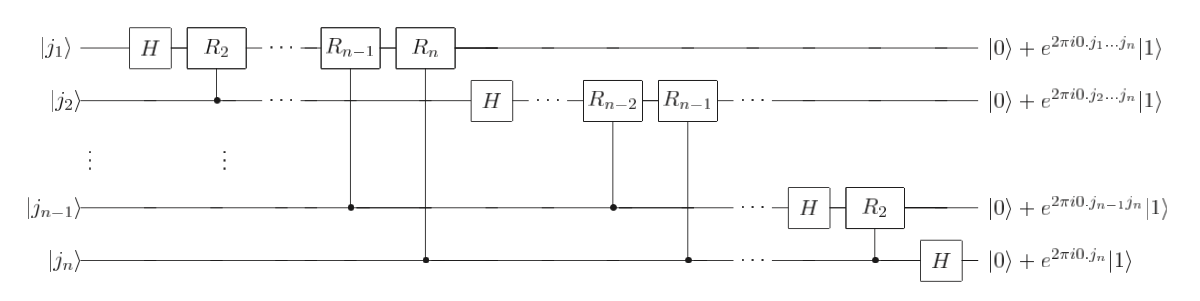
\includegraphics[width=1.0\textwidth]{fourier_circuit.png}
    \caption{Efficient circuit for the quantum Fourier transform.}
\end{figure}

\subsection{Phase estimation}

The Fourier transform is the key to a general procedure known as \textit{phase estimation}, which in turn is the key for many quantum algorithms. Suppose a unitary operator $U$ has an eigenvector $\ket{u}$ with eigenvalue $e^{2\pi i\phi}$, where the value of $\phi$ is unknown. The goal of the phase estimation algorithm is to estimate $\phi$. To do this, we will assume that we already have available some \textit{black boxes} capable of preparing the state $\ket{u}$ and performing the controlled-$U^2^j$ operation, for suitable non-negative integers $j$.
\vspace{1em}

The quantum phase estimation procedure uses two registers. The first register contains $t$ qubits initially in the state $\ket{0}$. How we choose $t$ depends on two things: the number of digits of accuracy we wish to have in our estimate for $\phi$, and with what probability we wish the phase estimation procedure to be successful. The second register begins in the state $\ket{u}$, and contains as many qubits as is necessary to store $\ket{u}$. Phase estimation is performed in two stages. First, we apply the circuit shown in the figure. The circuit begins by applying a Hadamard transform to the first register, followed by application of controlled-$U$ operations on the second register, with $U$ raised to successive powers of two. The final state of the first register is easily seen to be:
$$\frac{1}{2^{t/2}}\Big(\ket{0} + e^{2\pi i2^{t-1}\phi}\ket{1}\Big)\Big(\ket{0} + e^{2\pi i2^{t-2}\phi}\ket{1}\Big)\dots\Big(\ket{0} + e^{2\pi i2^{0}\phi}\ket{1}\Big)
= \frac{1}{2^{t/2}}\sum_{k=0}^{2^t-1}{e^{2\pi i\phi k}\ket{k}}$$
We omit the second register from this description, since it stays in the state $\ket{u}$ throughout the computation.
\begin{figure}[h]
    \centering
    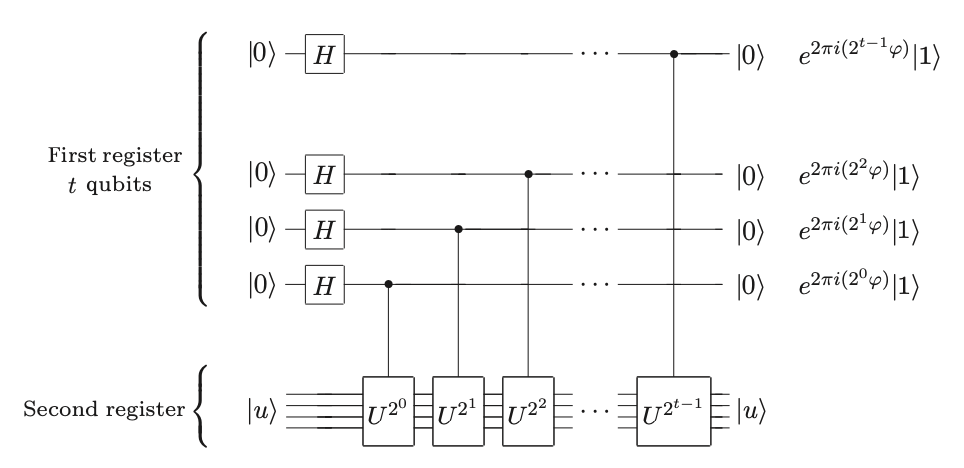
\includegraphics[width=1.0\textwidth]{phase_est.png}
    \caption{The first stage of the phase estimation procedure.}
\end{figure}
\vspace{1em}

The second stage of phase estimation is to apply the inverse quantum Fourier transform on the first register. This is obtained by reversing the circuit for the quantum Fourier transform, and can be done in $\Theta(t^2)$ steps. The third and final stage of phase estimation is to read out the state of the first register by doing a measurement in the computational basis. We will show that this provides a pretty good estimate of $\phi$. An overall schematic of the algorithm is shown below.
\begin{figure}[h]
    \centering
    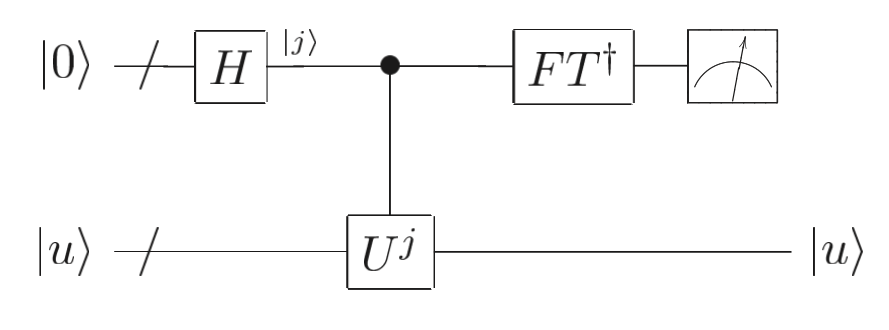
\includegraphics[width=0.8\textwidth]{overall_phase.png}
    \caption{Schematic of the overall phase estimation procedure.}
\end{figure}

\newpage
To see why phase estimation works, suppose $\phi$ may be expressed exactly in $t$ bits, as $\phi = 0.\phi_1\dots\phi_t$. Then the state resulting from the first stage of phase estimation may be rewritten
$$\frac{1}{2^{t/2}}\Big(\ket{0} + e^{2\pi i0.\phi_t}\ket{1}\Big)\Big(\ket{0} + e^{2\pi i0.\phi_{t-1}\phi_t}\ket{1}\Big)\dots\Big(\ket{0} + e^{2\pi i0.\phi_1\dots\phi_t}\ket{1}\Big)$$
The second stage of phase estimation is to apply the inverse quantum Fourier transform. But comparing the previous equation with the product form for the Fourier transform, we see that the output state from the second stage is the product state $\ket{\phi_1\dots\phi_t}$. A measurement in the computational basis therefore gives us $\phi$ exactly!

\subsection{Applications}

\subsubsection{Application: order-finding}

For positive integers $x$ and $N$ , $x < N$ , with no common factors, the \textit{order} of $x$ modulo $N$ is defined to be the least positive integer, $r$, such that $x^r = 1\ (mod\ N)$. The order-finding problem is to determine the order for some specified $x$ and $N$. Order-finding is believed to be a hard problem on a classical computer, in the sense that no algorithm is known to solve the problem using resources polynomial in the $O(L)$ bits needed to specify the problem, where $L \equiv \lceil\log(N)\rceil$ is the number of bits needed to specify $N$. In this section we explain how phase estimation may be used to obtain an efficient quantum algorithm for order-finding.
\vspace{1em}

The quantum algorithm for order-finding is just the phase estimation algorithm applied to the unitary operator
$$U\ket{y} \equiv \ket{xy\ (mod\ N)}$$
A simple calculation shows that the states defined by
$$\ket{u_s} \equiv \frac{1}{\sqrt{r}}\sum_{k=0}^{r-1}{\exp{\frac{-2\pi isk}{r}}\ket{x^k\ mod N}},$$
for integer $0 \le s \le r - 1$ are eigenstates of $U$, since
\begin{equation*}
\begin{split}
    U\ket{u_s} & = \frac{1}{\sqrt{r}}\sum_{k=0}^{r-1}{\exp{\frac{-2\pi isk}{r}}\ket{x^{k+1}\ mod N}}\\
    & = \exp{\frac{2\pi is}{r}}\ket{u_s}
\end{split}
\end{equation*}

Using the phase estimation procedure allows us to obtain, with high accuracy, the corresponding eigenvalues $\exp(2\pi is/r)$, from which we can obtain the order $r$ with a little bit more work.

\begin{figure}[h]
    \centering
    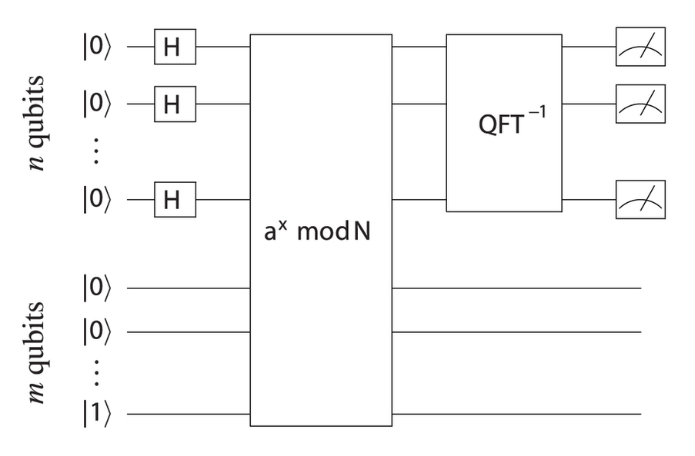
\includegraphics[width=0.8\textwidth]{order_finding.png}
    \caption{Circuit diagram for order finding algorithm.}
\end{figure}

\subsubsection{Application: factoring}

The \textit{factoring problem} goes as follows : given any integer $N$, find all of its prime factors and the exponent with which they appear. This factoring problem turns out to be equivalent to the order-finding problem in the sense that a fast algorithm for order-finding can easily be turned into a fast algorithm for factoring.
\vspace{1em}

The reduction of factoring to order-finding proceeds in two basic steps. The first step is to show that we can compute a factor of $N$ if we can find a non-trivial solution $x \neq \pm 1\ (mod\ N)$ to the equation $x^2 = 1\ (mod\ N)$. The second step is to show that a randomly chosen $y$ co-prime to N is quite likely to have an order $r$ which is even, and such that $y^{r/2} \neq \pm 1\ (mod\ N)$, and thus $x \equiv y^{r/2}\ (mod\ N)$ is a non-trivial solution to $x^2 = 1\ (mod\ N)$.

\begin{theorem}
    Suppose $N$ is an $L$ bit composite number, and $x$ is a non-trivial solution to the equation $x^2 = 1\ (mod\ N)$ in the range $1 \le x \le N$, that is, neither $x = 1\ (mod\ N)$ nor $x = N - 1 = -1\ (mod\ N)$. Then at least one of $\gcd(x - 1,N)$ and $\gcd(x + 1,N)$ is a non-trivial factor of $N$ that can be computed using $O(L^3)$ operations.
\end{theorem}
\begin{theorem}
    Suppose $N = p_1^{\alpha 1}\dots p_m^{\alpha_m}$ is the prime factorization of an odd composite positive integer. Let $x$ be an integer chosen uniformly at random, subject to the requirements that $1 \le x \le N - 1$ and $x$ is co-prime to $N$. Let $r$ be the order of $x$ modulo $N$. Then
    $$p(r\textnormal{ is even and }x^{r/2} \neq -1\ (mod\ N)) \geq 1 - \frac{1}{2^m}$$
\end{theorem}

Above theorems can be combined to give an algorithm which, with high probability, returns a non-trivial factor of any composite $N$. All the steps in the algorithm can be performed efficiently on a classical computer except (so far as is known today) an order-finding 'subroutine' which is used by the algorithm. By repeating the procedure we may find a complete prime factorization of $N$. The algorithm is summarized below.
\vspace{1em}

\textbf{Algorithm: Reduction of factoring to order-finding}
\begin{quote}
    \textbf{Inputs:} A composite number $N$.\\
    \textbf{Outputs:} A non-trivial factor of $N$.\\
    \textbf{Runtime:} $O((\log N)^3)$ operations. Succeeds with probability $O(1)$.\\
    \textbf{Procedure:}
    \begin{enumerate}
        \item If $N$ is even, return the factor $2$.
        \item Determine whether $N = a^b$ for integers $a \geq 1$ and $b \geq 2$, and if so return the factor $a$.
        \item Randomly choose $x$ in the range $1$ to $N-1$. If $\gcd(x,N) > 1$ then return the factor $\gcd(x,N)$.
        \item Use the order-finding subroutine to find the order $r$ of $x$ modulo $N$.
        \item If $r$ is even and $x^{r/2} \neq -1\ (mod\ N)$ then compute $\gcd(x^{r/2}-1,N)$ and $\gcd(x^{r/2} + 1, N)$, and test to see if one of these is a non-trivial factor, returning that factor if so. Otherwise, the algorithm fails.
    \end{enumerate}
\end{quote}

\newpage
\subsubsection{Application : Period-finding}

Consider the following problem. Suppose $f$ is a periodic function producing a single bit as output and such that $f(x + r) = f(x)$, for some unknown $0 < r < 2L$, where $x, r \in \{0, 1, 2, \dots\}$. Given a quantum black box $U$ which performs the unitary transform $U\ket{x}\ket{y} \rightarrow \ket{x}\ket{y \oplus f(x)}$ (where $\oplus$ denotes addition modulo $2$) how many black box queries and other operations are required to determine $r$? Note that in practice $U$ operates on a finite domain, whose size is determined by the desired accuracy for $r$. Here is a quantum algorithm which solves this problem using one query, and $O(L^2)$ other operations:\\
\textbf{Algorithm: Period-finding}
\begin{quote}
    \textbf{Inputs:} (1) A black box which performs the operation $U\ket{x}\ket{y} = \ket{x}\ket{y \oplus f(x)}$, (2) a state to store the function evaluation, initialized to $\ket{0}$, and (3) $t = O(L + \log(1/\epsilon))$ qubits initialized to $\ket{0}$.\\
    \textbf{Outputs:} The least integer $r > 0$ such that $f(x + r) = f(x)$.\\
    \textbf{Runtime:} One use of $U$, and $O(L^2)$ operations. Succeeds with probability $O(1)$.\\
    \textbf{Procedure:}
    \begin{figure}[h]
        \centering
        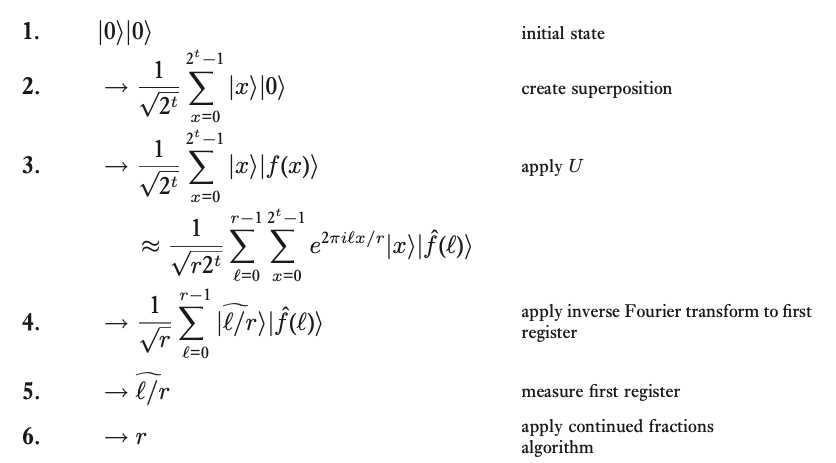
\includegraphics[width=0.9\textwidth]{period_algo.png}
    \end{figure}
\end{quote}
% The circuit diagram for period finding algorithm is as follows.
% \begin{figure}[h]
%     \centering
%     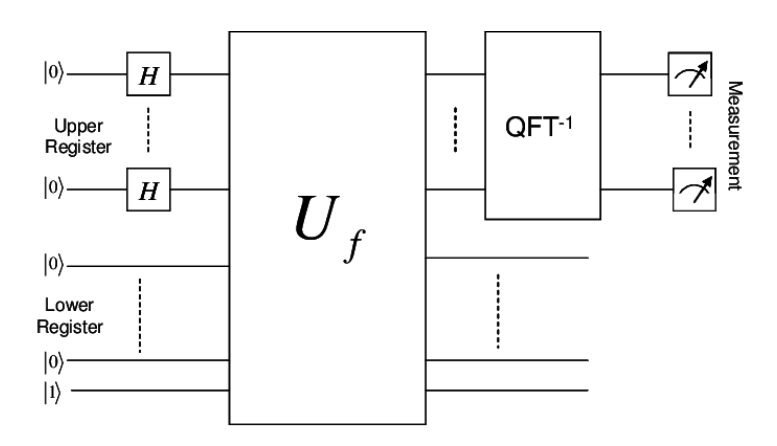
\includegraphics[width=0.8\textwidth]{period_circuit.png}
%     \caption{Circuit diagram for period finding algorithm.}
% \end{figure}